\clearpage
\section{Continuous Variable QKD Transmission System}\label{sec:intro}

\begin{tcolorbox}	
\begin{tabular}{p{2.75cm} p{0.2cm} p{10.5cm}} 	
\textbf{Student Name}  &:& Daniel Pereira (2017/05/01 - )\\
\textbf{Goal}          &:& Simulation and experimental validation of a CV-QKD transmission system.\\
\textbf{Directory}              &:& sdf/cv\_system  
\end{tabular}
\end{tcolorbox}

The aim of Continuous Variable Quantum Key Distribution (CV-QKD) is to encode information in observables whose measurements take continuous values.
\par
The purpose of this study is to analyse a CV-QKD transmission system in which the information is sent in the two orthogonal quadratures of a coherent state. 

\subsection{Theoretical Analysis}

The security of QKD is a complex topic to tackle, given the difficulty of proving the non-existence of an attack that cracks a protocol's security. This topic is usually approached by analysing various eavesdropping strategies and evaluating their effects on the key rate referenced in~\eqref{eq:keyrateperfect}. Information between Alice and Bob needs to be shared with current existing technology, so their shared information is always classical and Shannon's formalism is enough to describe it. However, Eve has no such restriction, so the information she has on Bob's results needs to be described according to the quantum properties of the system. 

\subsection{Simulation Analysis}

\begin{figure}[h]
\centering
%left bottom right top
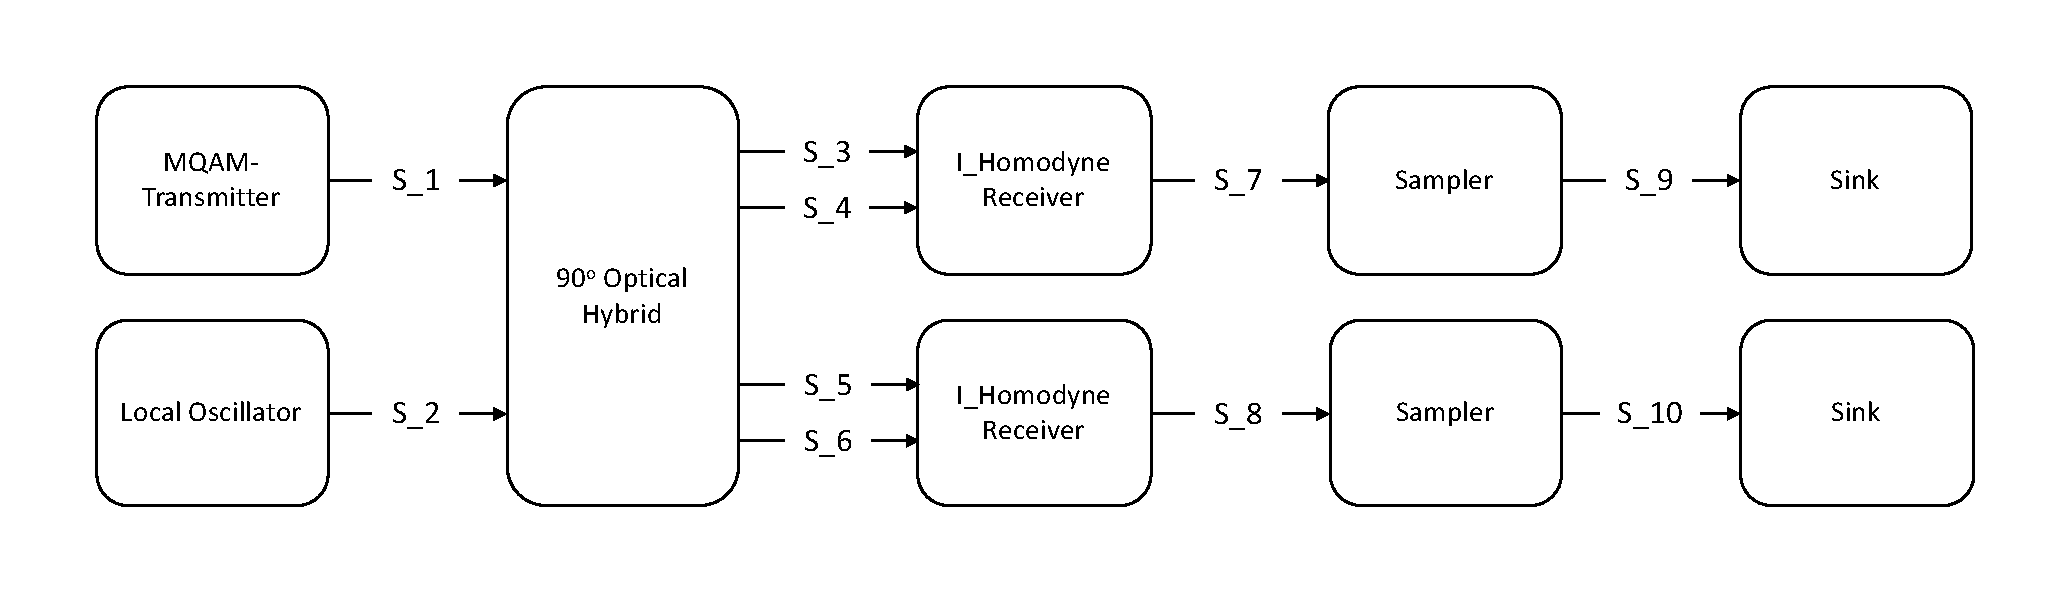
\includegraphics[width=\linewidth]{diagramSIMU.pdf}
\caption{Overview of the CV-QKD system being simulated.}
\label{fig:CV-System}
\end{figure}

\subsection*{Required files}\label{Required files}

\begin{table}[H]
\centering
\begin{tabulary}{1.0\textwidth}{|p{6cm}|p{8cm}|p{1cm}|}
\hline
\multicolumn{3}{|c|}{ \textbf{Header Files} } \\
\hline
\textbf{File}                    & \textbf{Comments}          & \textbf{Status} \\ \hline
add.h                            &                            & \checkmark \\ \hline
binary\_source.h                 &                            & \checkmark \\ \hline
discrete\_to\_continuous\_time.h &                            & \checkmark \\ \hline
i\_homodyne\_reciever.h          & Working, but bootstrapped. & \checkmark \\ \hline
ideal\_amplififer.h              &                            & \checkmark \\ \hline
iq\_modulator.h                  &                            & \checkmark \\ \hline
local\_oscillator.h              &                            & \checkmark \\ \hline
m\_qam\_mapper.h                 &                            & \checkmark \\ \hline
m\_qam\_transmitter.h            &                            & \checkmark \\ \hline
netxpto.h                        &                            & \checkmark \\ \hline
optical\_hybrid.h                &                            & \checkmark \\ \hline
photodiode.h                     & Currently being rewritten. &  \\ \hline
pulse\_shaper.h                  &                            & \checkmark \\ \hline
sampler.h                        &                            & \checkmark \\ \hline
sink.h                           &                            & \checkmark \\ \hline
super\_block\_interface.h        &                            & \checkmark \\ \hline
white\_noise.h                   &                            & \checkmark \\ \hline
\end{tabulary}
\end{table}		
%
\begin{table}[H]
\centering
\begin{tabulary}{1.0\textwidth}{|p{6cm}|p{8cm}|p{1cm}|}
\hline
\multicolumn{3}{|c|}{ \textbf{Source Files} } \\
\hline
\textbf{File}                      & \textbf{Comments}          & \textbf{Status} \\ \hline
add.cpp                            &                            & \checkmark \\ \hline
binary\_source.cpp                 &                            & \checkmark \\ \hline
discrete\_to\_continuous\_time.cpp &                            & \checkmark \\ \hline
i\_homodyne\_reciever.cpp          & Working, but bootstrapped. & \checkmark \\ \hline
ideal\_amplififer.cpp              &                            & \checkmark \\ \hline
iq\_modulator.cpp                  &                            & \checkmark \\ \hline
local\_oscillator.cpp              &                            & \checkmark \\ \hline
m\_qam\_mapper.cpp                 &                            & \checkmark \\ \hline
m\_qam\_transmitter.cpp            &                            & \checkmark \\ \hline
netxpto.cpp                        &                            & \checkmark \\ \hline
optical\_hybrid.cpp                &                            & \checkmark \\ \hline
photodiode.cpp                     & Currently being rewritten. &  \\ \hline
pulse\_shaper.cpp                  &                            & \checkmark \\ \hline
sampler.cpp                        &                            & \checkmark \\ \hline
sink.cpp                           &                            & \checkmark \\ \hline
super\_block\_interface.cpp        &                            & \checkmark \\ \hline
white\_noise.cpp                   &                            & \checkmark \\ \hline
\end{tabulary}
\end{table}		

\subsection*{System Input Parameters}

This system takes into account the following input parameters:

\begin{table}[H]
\centering
\begin{tabulary}{1.0\textwidth}{|p{6cm}|p{4cm}|p{5cm}|}
\hline
\multicolumn{3}{|c|}{ \textbf{System Input Parameters} } \\
\hline
\textbf{Parameter}     & \textbf{Default Value}                                     & \textbf{Comments} \\ \hline
numberOfBitsGenerated  & $40000$	                                                   &                     \\ \hline
bitPeriod              & $20\times10^{-12}$                                         &\\ \hline
samplesPerSymbol       & $16$                                                       &\\ \hline
pLength                & $5$                                                        &\\ \hline
iqAmplitudesValues     & $\lbrace~\lbrace-1,~0\rbrace~,~\lbrace1,~0\rbrace~\rbrace$ & \\ \hline
outOpticalPower\_dBm   & Variable                                                   & Value varied for presented study\\ \hline
loOutOpticalPower\_dBm & $0$                                                        & \\ \hline
localOscillatorPhase   & $0$                                                        & \\ \hline
transferMatrix         & $\lbrace~\lbrace \frac{1}{\sqrt{2}},~\frac{1}{\sqrt{2}},~\frac{1}{\sqrt{2}},~\frac{-1}{\sqrt{2}} \rbrace~\rbrace$ & \\ \hline
responsivity           & $1$                                                        & \\ \hline
amplification          & $10^3$                                                     & \\ \hline
noiseSpectralDensity   & $5\times10^{-4}\sqrt{2}$~V$^2$                             & \\ \hline
confidence             & $0.95$                                                     & \\ \hline
midReportSize          & $0$                                                        & \\ \hline
\end{tabulary}
\end{table}		

\subsection*{Inputs}

This system takes no inputs.

\subsection*{Outputs}

This system outputs the following objects:
\begin{itemize}
\item Signals:
\begin{itemize}
\item Optical Signal with coded Binary String; (S$_{1}$)
\item Local Oscillator Optical Signal; (S$_{2}$)
\item 90$^\text{o}$ Optical Hybrid Outputs; (S$_{3}$, S$_{4}$, S$_{5}$, S$_{6}$)
\item Homodyne Detectors' Electrical Output; (S$_{7}$, S$_{8}$)
\item Sampled Signals; (S$_{9}$, S$_{10}$)
\end{itemize}
\end{itemize}

\subsection{Comparative Analysis}

\bibliographystyle{unsrt}
 
\bibliography{bibliography}
